\section{Korrelationsmatrizen sortiert nach dem Gemeindeschlüssel}
\subsection{Korrelationsmatrizen mit den nach Gemeindeschlüsseln sortierten Landkreise}
In \autoref{fig:matrizes_north_to_south_counties} befinden sich die sechs Matrizen mit den Werten für die Korrelationen zwischen den Landkreisen.
Die Zeilen und Spalten sind lexikographisch nach den Gemeindeschlüsseln der Landkreise sortiert, dies entspricht in etwa einem Nord-Süd-Verlauf (siehe \autoref{fig:distribution_AdmUnitId}). Im Anhang in \autoref{tab:counties_by_admunitid} befindet sich die vollständige Auflistung.

\begin{figure}[H]
    \centering
    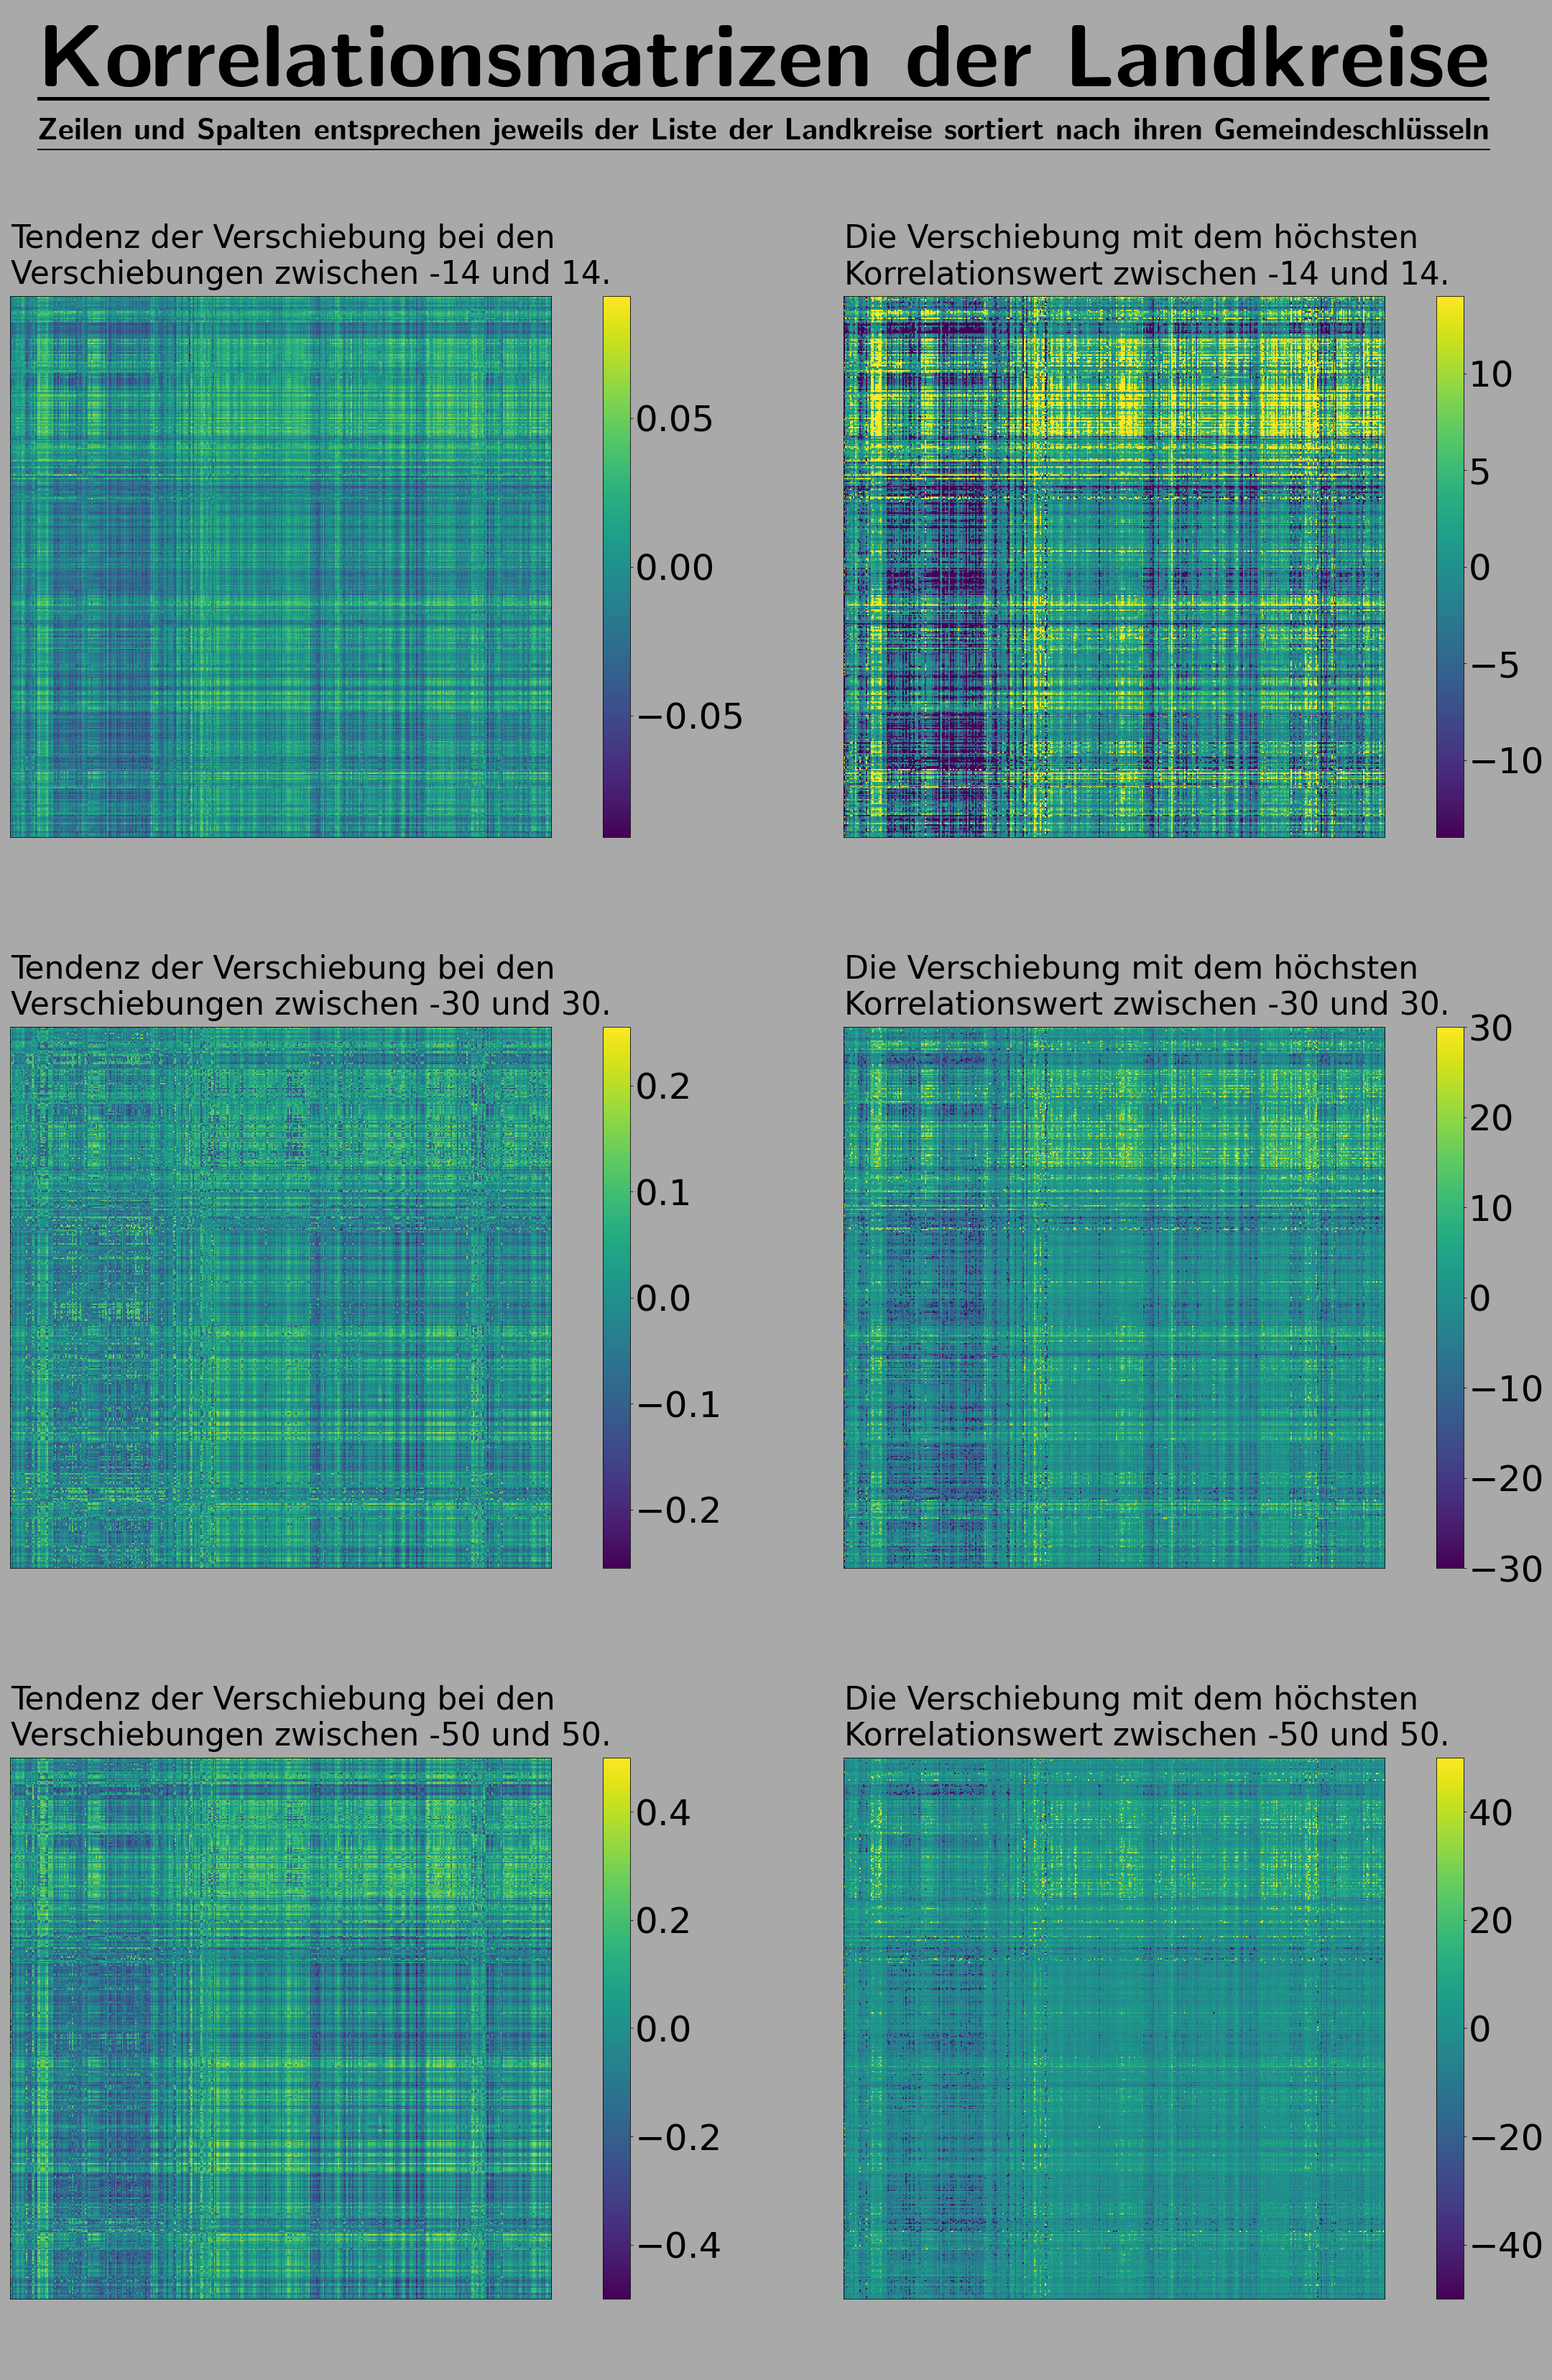
\includegraphics[width = 0.75\textwidth]{figures/Ergebnisse/matrizes_north_to_south_counties.png}
    \caption{Korrelationsmatrizen der Korrelationen aller Landkreise zeilen- und spaltenweise nach dem Gemeindeschlüssel sortiert (siehe \autoref{tab:counties_by_admunitid}). Die Farben der Zellen der linken Matrizen entsprechen den Tendenzen der Verschiebung des Landkreises der Spalte in Relation zum Landkreis der Zeile.
    Auf der rechten Seite wir die Zelle entsprechend der Verschiebung der Zeitserie des Landkreises der Spalte entgegen der Zeitserie der Zeile mit dem höchsten Korrelationswert eingefärbt. Beide Vorgehensweise werden für alle ganzzahligen Verschiebungen $\tau\in[-14,14]$,  $\tau\in[-30,30]$ und  $\tau\in[-50,50]$ durchgeführt und in dieser Reihenfolge von oben nach unten dargestellt.}
    \label{fig:matrizes_north_to_south_counties}
\end{figure}
\subsection{Korrelationsmatrizen mit den nach Gemeindeschlüsseln sortierten Regierungsbezirken}
Die sechs Matrizen mit den Werten für die Korrelationen zwischen den Regierungsbezirken befinden sich in \autoref{fig:matrizes_north_to_south_districts} . Auch hier sind die Zeilen und Spalten lexikographisch nach den Gemeindeschlüsseln der Landkreise in den Regierungsbezirken sortiert. Die vollständige Auflistung von diesen befindet sich im Anhang in \autoref{tab:districts_by_admunitid}.

\begin{figure}[H]
    \centering
    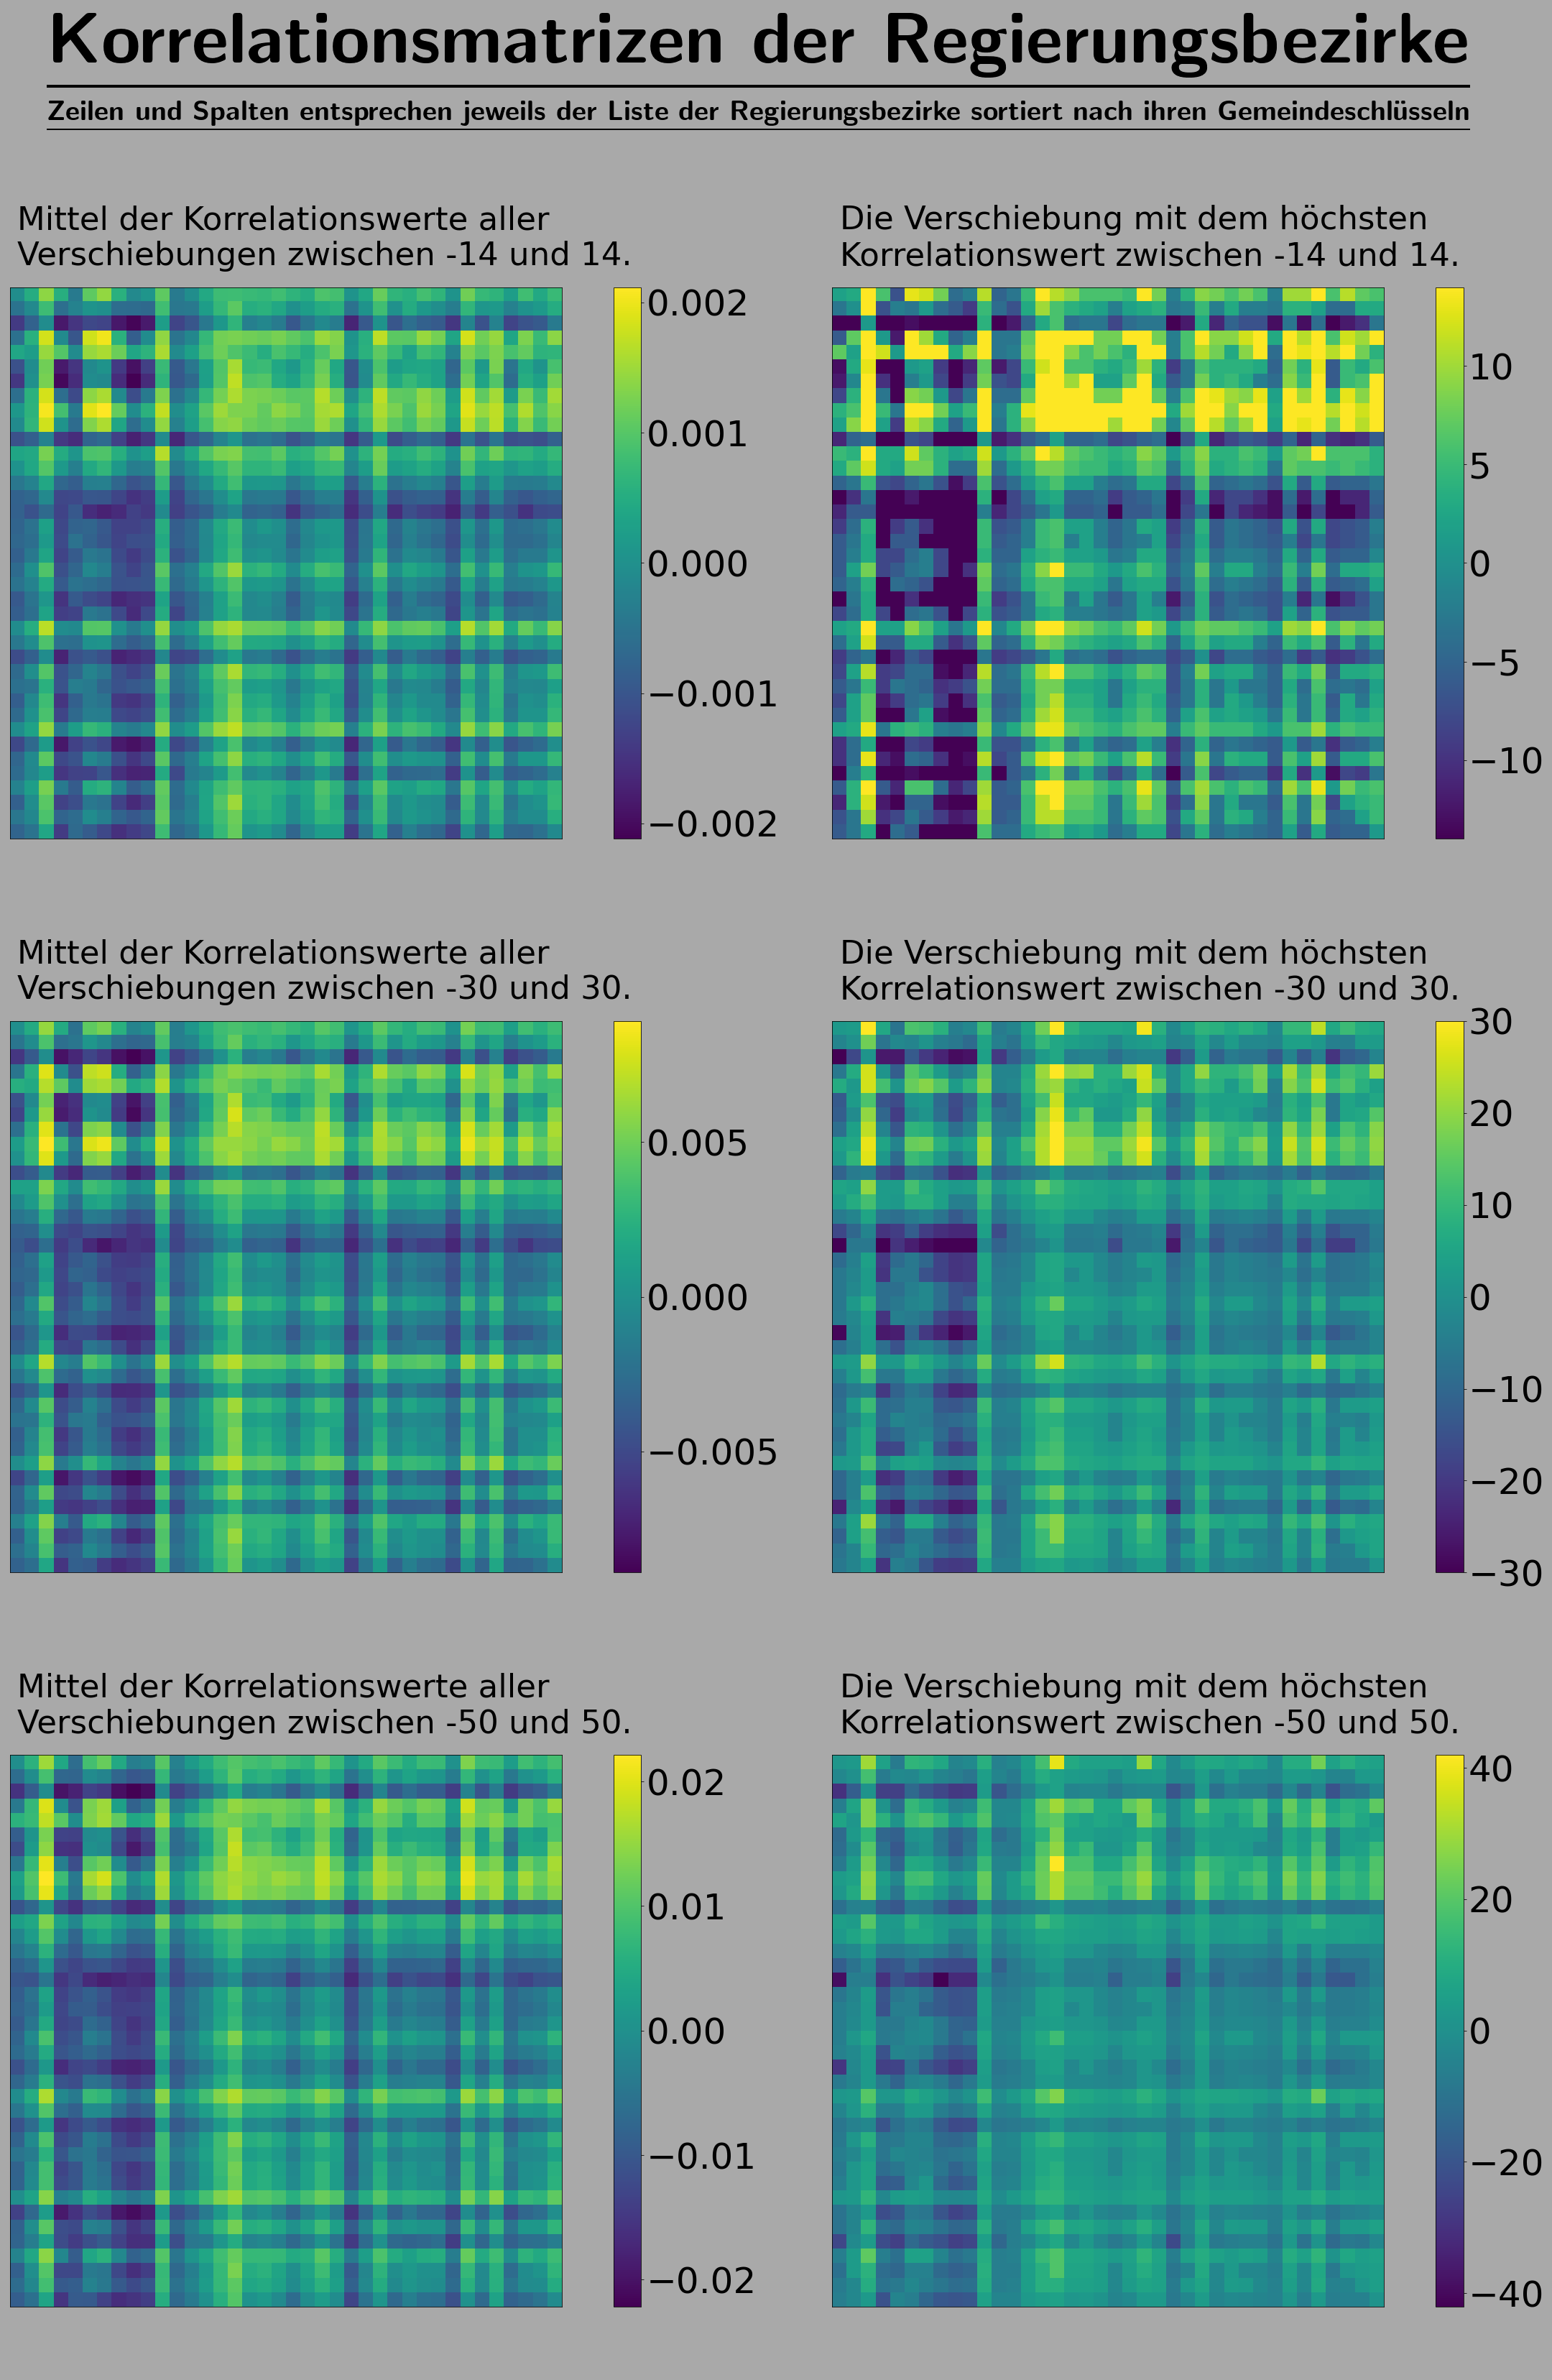
\includegraphics[width = 0.75\textwidth]{figures/Ergebnisse/matrizes_north_to_south_districts.png}
    \caption{Korrelationsmatrizen der Korrelationen aller Regierungsbezirke zeilen- und spaltenweise nach dem Gemeindeschlüssel sortiert (siehe \autoref{tab:districts_by_admunitid}). Die Farben der Zellen der linken Matrizen entsprechen den Tendenzen der Verschiebung des Regierungsbezirks der Spalte in Relation zum Regierungsbezirks der Zeile.
    Auf der rechten Seite wir die Zelle entsprechend der Verschiebung der Zeitserie des Regierungsbezirks der Spalte entgegen der Zeitserie der Zeile mit dem höchsten Korrelationswert eingefärbt. Beide Vorgehensweise werden für alle ganzzahligen Verschiebungen $\tau\in[-14,14]$,  $\tau\in[-30,30]$ und  $\tau\in[-50,50]$ durchgeführt und in dieser Reihenfolge von oben nach unten dargestellt.}
    \label{fig:matrizes_north_to_south_districts}
\end{figure}
